\documentclass{article}
\usepackage[margin=2cm]{geometry}
\usepackage{float}
\usepackage{graphicx}
\usepackage{hyperref}


% Paragraph settings
\setlength{\parskip}{10pt plus 1pt minus 1pt
\setlength{\parindent}{0cm}}

\begin{document}
\title{CS22310 - Hotel Site Assignment}
\author{Samuel Jackson \\ \texttt{slj11@aber.ac.uk}}
\date{\today}
\maketitle

\section{Introduction}
This document provides the final report for the CS22310 Hotel Site assignment and contains the task analysis, interaction design, documentation of prototype and discussion of usability principles. The prototype implementation for this site can be found at \url{http://users.aber.ac.uk/slj11/cs22310/index.html}

\section{Task Analysis}
This section of the document details the analysis of the brief and the identification for the major tasks that the system needs to perform along with characterisation of the users that will perform these tasks. The analysis is documented using a rich picture, use case, data flow and state transition diagrams along with an accompanying description of each.

\subsection{Identification of Users}
For the first step in my task analysis, I created a rich picture to provide a high level overview of the proposed system and try and identify its major functions and users.

\begin{figure}[H]
\centering
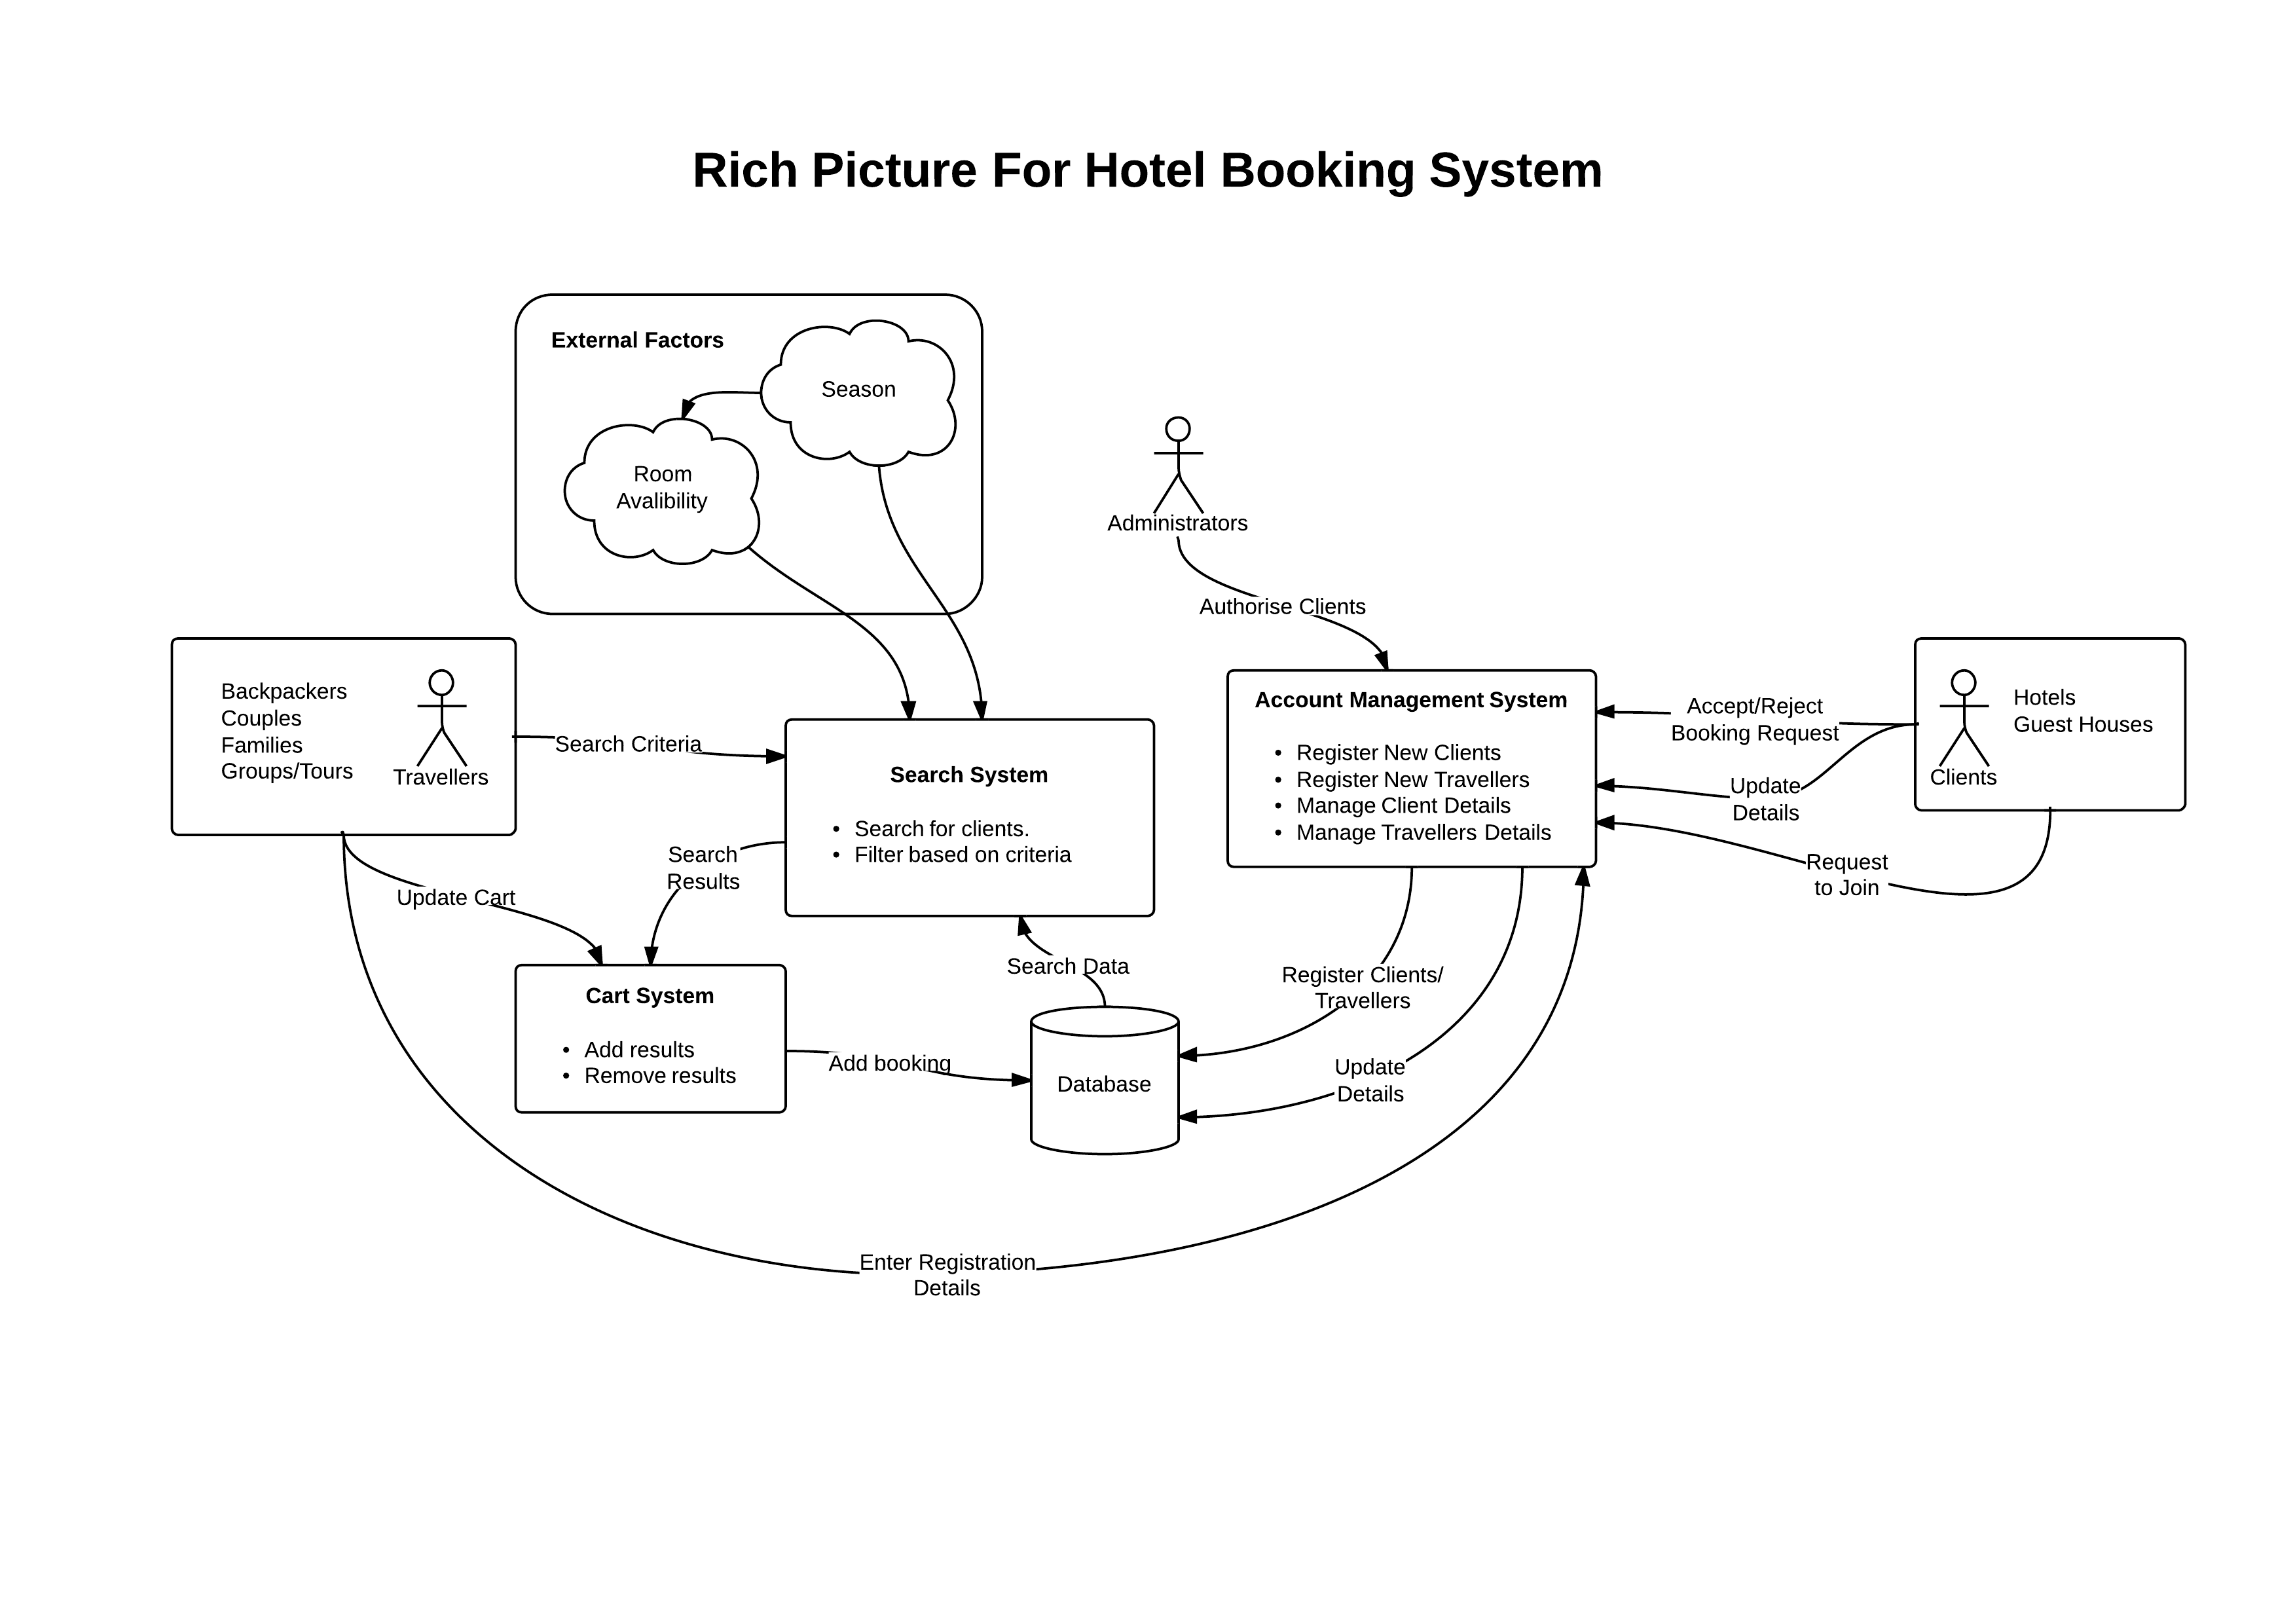
\includegraphics[width=1\textwidth]{img/richpic.png}
\caption{Rich Picture for the Hotel Site}
\label{fig:rich-pic}
\end{figure}

In this diagram, I have identified three key users of the system and three major "task areas" that our system must be able to perform. The major actors in the system are as follows:
\begin{itemize}
	\item \textbf{Travellers} - Travellers are customers of the hotel booking site who wish to search and book lodging with the hotels and guest houses listed on the site.
	\item \textbf{Clients} - Clients are also customers of the hotel booking site, but are representatives or managers of various hotels and guest houses which can register an account with the site to list there available accommodation.
	\item \textbf{Administrators} - Administrators are employees of the hotel booking site and who's only major function is to authorise requests by clients for registration with the site.
\end{itemize}

Of the three major types of users identified here, the most technologically inexperienced are most likely to be the Travellers. This is due to the potentially wide variety of different customers that could use the site as this a diverse user demographic implies a wide diversity in technological competency. They  will also have almost no training in how to use the system (unlike administrators and possibly clients). It is therefore paramount that system functions undertaken by Travellers be as clear and accessible as possible. Travellers may be either single contact (they only use the site once) or may be repeat customers. Therefore there interface should accommodate inexperienced "first time" users while still providing ease of access for power users.

Clients are likely to be similar to travellers, but perhaps with slightly less diversity in competency. This is due to the fact that the hotel/guest house may have a dedicated member of staff (such as a manager) that is responsible for dealing with the management of hotel's listing on the site. This employee may also receive training by an employee which already knows how to use the system. However, when a new client registers with the hotel site, the client management interface stills needs to be intuitive to the first time users. This point is particularly relevant the smaller hotels and guest houses who are more likely to not have a technical professional to handle the establishments web presence.

Client will have a recurring connection with hotel site and there connection is most likely going to last for months and years, rather than being a single one off connection with the site like some potential Travellers. Again it is stressed that this section of the site be accessible to a variety of user skill levels. It is also more of a requirement that this part of the site be efficient. Client users are not looking to "browse" like Travellers but are coming to the site to perform a specific task (e.g. updating promotional information) and therefore want clear and easy to use interface to quick accomplish the task the came to do.

The final major type of system user are administrators. Administrators are likely to be the most technically competent users. They are expected to have frequent, recurrent contact with the system, probably on a daily basis. They are also likely to be well trained by the company running the hotel booking site. Like Clients, they will not wish to "browse" the site, but will come to it in order to carry out a specific task and therefore will want a clear and efficient interface suitable for a power user.

The rich picture also identifies three key categories that user tasks fall into across the site. The first category of task are those related to the management of the accounts associated with users. This includes tasks that allow the Clients to update information about their establishment, the registration of Client and Travellers and Travellers updating their payment and billing information. Task in this category are carried out by each of the types of system users.

In contrast, the other two categories that system tasks fall into are only carried out by Travellers. These two areas are the search system and the cart/payment system. Both of these areas are distinct but closely related. In fact, the search system feeds into the cart and payment system. However, the search system is concerned with getting results that match the users criteria and refining there choices. The cart system is designed to guide the user through the payment and booking process after they have finished making their choices. Note that the picture also displays some external influences on the search system which ma affect the results available to Travellers, such as room availability and the season.

As a final note, I have also added the a data store labelled database. This is the major data sink on the hotel site server where information about bookings, hotel and user accounts all feed into. Data is pulled from this store and displayed via the interface as required.

\subsection{System Tasks}

\subsection{Data Flow Diagram}

\subsection{State Transition Diagrams}

\section{Interaction Design}

\section{Prototype}

\section{Discussion}
\end{document}